\chapter{2D Nominal Monte-Carlo Distributions, 2018}
\label{chap:nominal_mc_2018}

\section{FGD1 $\nu_\mu$ FHC}
\autoref{fig:nominal2D_FGD1numu_2018} shows the data and nominal model prediction for the FGD1 FHC selections. We see in the restricted plotting region (excluding highest momentum and most backward bins, normalising to bin width), the data is consistently higher than the prediction. The CC0$\pi$ selection looks overestimated at higher momentum between \cosmu=0.8-0.95. We also see some clear underestimates along lines of constant $Q^2$, between 0.07 and 0.15 $\text{GeV}^2$. For the CC1$\pi$ selection we see a similar overestimate at high \pmu and \cosmu=0.8-0.95. For the CCOther selection we see a clear underestimate in almost all bins below $Q^2=0.2\text{ GeV}^2$. In general, the distributions are compatible and similar to the 2017 equivalents in \autoref{fig:nominal2D_FGD1numu}.
\begin{figure}[h]
	\begin{subfigure}[t]{0.32\textwidth}
		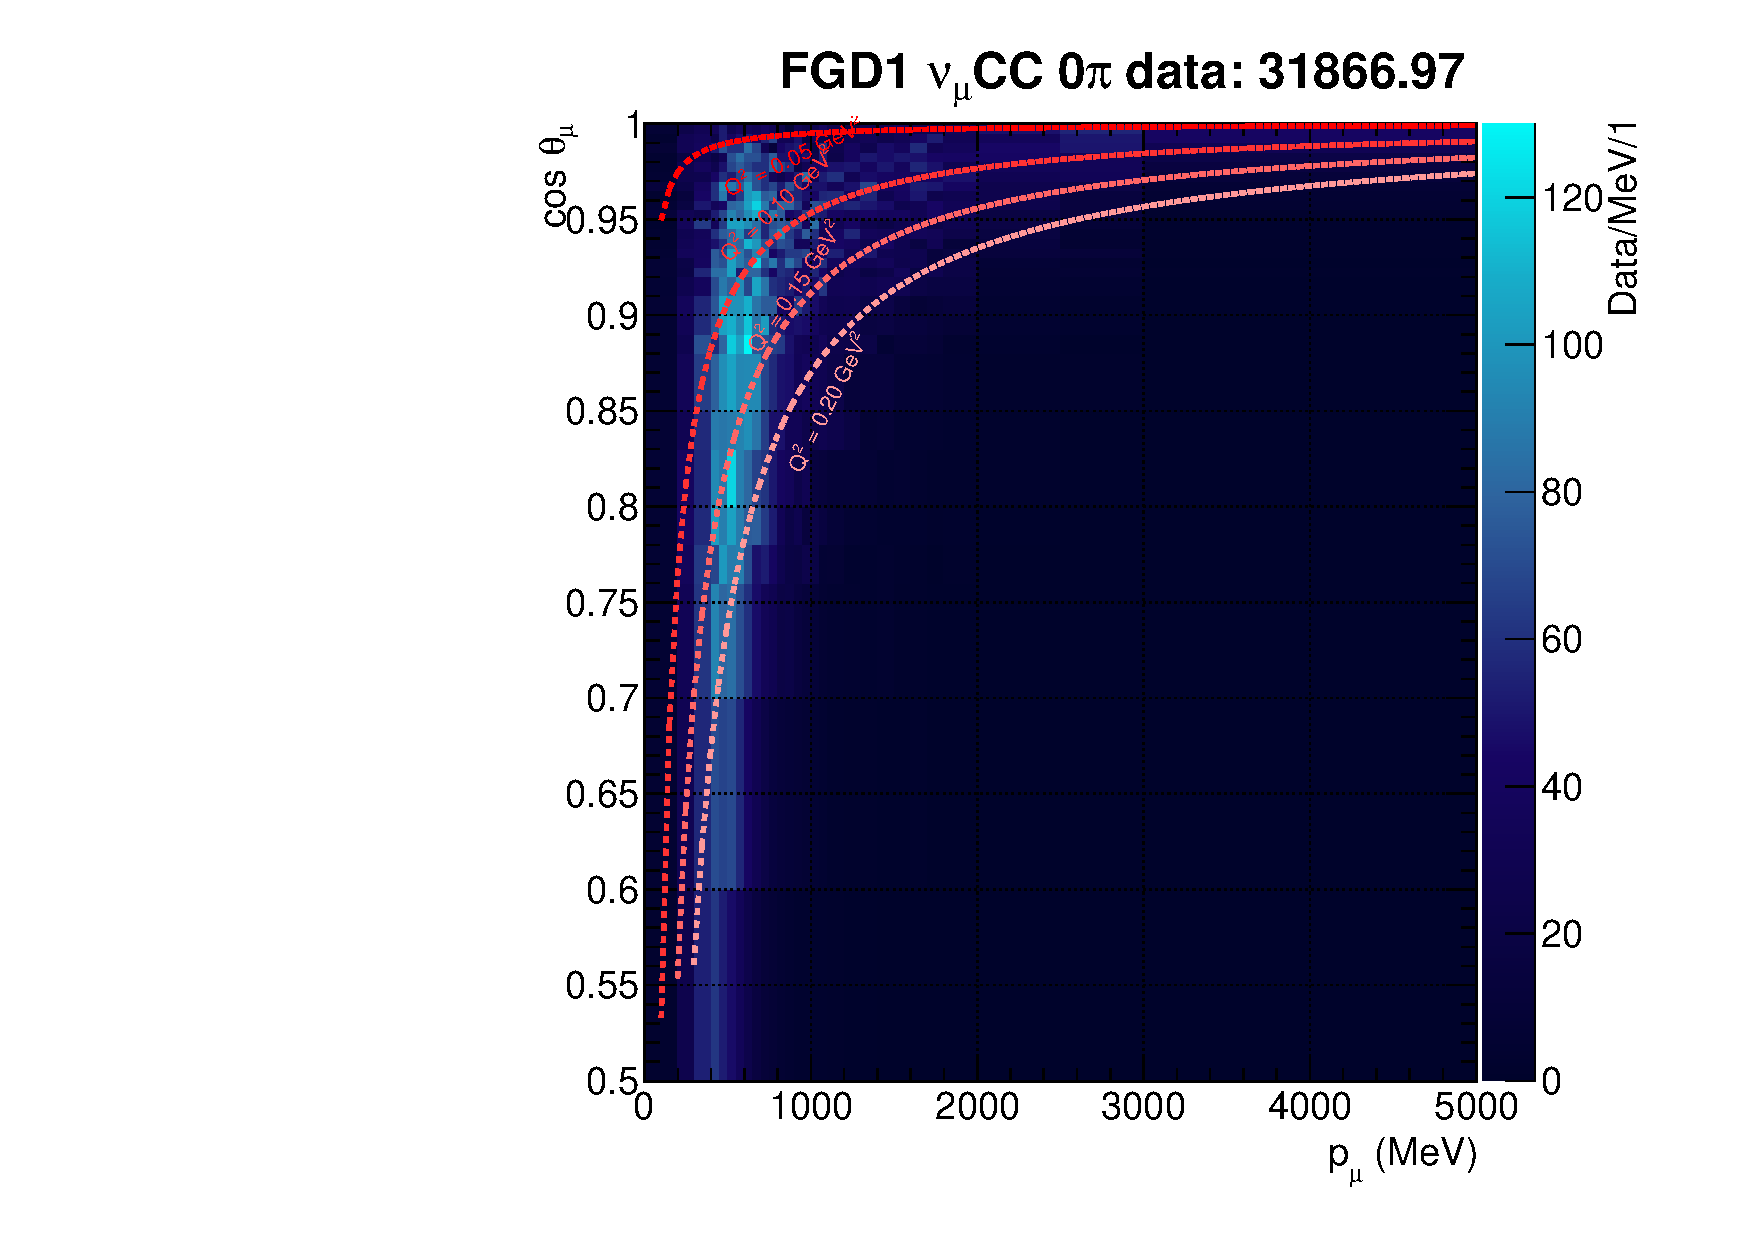
\includegraphics[width=\textwidth,page=1]{{figures/mach3/2018/Selection/2018_RedNDmatrix_rebin_verbose_may_noweights_ND280_nom}}
	\end{subfigure}
	\begin{subfigure}[t]{0.32\textwidth}
		\includegraphics[width=\textwidth,page=2]{{figures/mach3/2018/Selection/2018_RedNDmatrix_rebin_verbose_may_noweights_ND280_nom}}
	\end{subfigure}
	\begin{subfigure}[t]{0.32\textwidth}
		\includegraphics[width=\textwidth,page=3]{{figures/mach3/2018/Selection/2018_RedNDmatrix_rebin_verbose_may_noweights_ND280_nom}}
	\end{subfigure}
	
	\begin{subfigure}[t]{0.32\textwidth}
		\includegraphics[width=\textwidth,page=4]{{figures/mach3/2018/Selection/2018_RedNDmatrix_rebin_verbose_may_noweights_ND280_nom}}
	\end{subfigure}
	\begin{subfigure}[t]{0.32\textwidth}
		\includegraphics[width=\textwidth,page=5]{{figures/mach3/2018/Selection/2018_RedNDmatrix_rebin_verbose_may_noweights_ND280_nom}}
	\end{subfigure}
	\begin{subfigure}[t]{0.32\textwidth}
		\includegraphics[width=\textwidth,page=6]{{figures/mach3/2018/Selection/2018_RedNDmatrix_rebin_verbose_may_noweights_ND280_nom}}
	\end{subfigure}
	
	\begin{subfigure}[t]{0.32\textwidth}
		\includegraphics[width=\textwidth,page=7]{{figures/mach3/2018/Selection/2018_RedNDmatrix_rebin_verbose_may_noweights_ND280_nom}}
	\end{subfigure}
	\begin{subfigure}[t]{0.32\textwidth}
		\includegraphics[width=\textwidth,page=8]{{figures/mach3/2018/Selection/2018_RedNDmatrix_rebin_verbose_may_noweights_ND280_nom}}
	\end{subfigure}
	\begin{subfigure}[t]{0.32\textwidth}
		\includegraphics[width=\textwidth,page=9]{{figures/mach3/2018/Selection/2018_RedNDmatrix_rebin_verbose_may_noweights_ND280_nom}}
	\end{subfigure}
	
	\caption{Data and nominal MC distributions and the Data/MC ratio for FGD1 FHC selections. Lines of constant $Q^2_\text{reco}$ are shown. Bin content is normalised to bin width.}
	\label{fig:nominal2D_FGD1numu_2018}
\end{figure}

\section{FGD2 $\nu_\mu$ FHC}
\autoref{fig:nominal2D_FGD2numu_2018} shows the nominal FHC \numu distributions for FGD2, with very similar behaviour to the FGD1 distributions.
\begin{figure}[h]
	\begin{subfigure}[t]{0.32\textwidth}
		\includegraphics[width=\textwidth,page=10]{{figures/mach3/2018/Selection/2018_RedNDmatrix_rebin_verbose_may_noweights_ND280_nom}}
	\end{subfigure}
	\begin{subfigure}[t]{0.32\textwidth}
		\includegraphics[width=\textwidth,page=11]{{figures/mach3/2018/Selection/2018_RedNDmatrix_rebin_verbose_may_noweights_ND280_nom}}
	\end{subfigure}
	\begin{subfigure}[t]{0.32\textwidth}
		\includegraphics[width=\textwidth,page=12]{{figures/mach3/2018/Selection/2018_RedNDmatrix_rebin_verbose_may_noweights_ND280_nom}}
	\end{subfigure}
	
	\begin{subfigure}[t]{0.32\textwidth}
		\includegraphics[width=\textwidth,page=13]{{figures/mach3/2018/Selection/2018_RedNDmatrix_rebin_verbose_may_noweights_ND280_nom}}
	\end{subfigure}
	\begin{subfigure}[t]{0.32\textwidth}
		\includegraphics[width=\textwidth,page=14]{{figures/mach3/2018/Selection/2018_RedNDmatrix_rebin_verbose_may_noweights_ND280_nom}}
	\end{subfigure}
	\begin{subfigure}[t]{0.32\textwidth}
		\includegraphics[width=\textwidth,page=15]{{figures/mach3/2018/Selection/2018_RedNDmatrix_rebin_verbose_may_noweights_ND280_nom}}
	\end{subfigure}
	
	\begin{subfigure}[t]{0.32\textwidth}
		\includegraphics[width=\textwidth,page=16]{{figures/mach3/2018/Selection/2018_RedNDmatrix_rebin_verbose_may_noweights_ND280_nom}}
	\end{subfigure}
	\begin{subfigure}[t]{0.32\textwidth}
		\includegraphics[width=\textwidth,page=17]{{figures/mach3/2018/Selection/2018_RedNDmatrix_rebin_verbose_may_noweights_ND280_nom}}
	\end{subfigure}
	\begin{subfigure}[t]{0.32\textwidth}
		\includegraphics[width=\textwidth,page=18]{{figures/mach3/2018/Selection/2018_RedNDmatrix_rebin_verbose_may_noweights_ND280_nom}}
	\end{subfigure}
	
	\caption{Data and nominal MC distributions and the Data/MC ratio for FGD2 FHC selections. Lines of constant $Q^2_\text{reco}$ are shown. Bin content is normalised to bin width.}
	\label{fig:nominal2D_FGD2numu_2018}
\end{figure}

\section{FGD1 $\bar{\nu}_\mu$ RHC}
\autoref{fig:nominal2D_FGD1numubar_2018} shows the first light for the new RHC CC0$\pi$, CC1$\pi$ and CCNTrack selections. The CC0$\pi$ selection is slightly over-estimated, but the nominal prediction looks more compatible with data than the FHC \numu distributions. The Data/MC ratio also doesn't appear to contain the same deficiency in $Q^2$. The CC1$\pi$ distribution is consistently underestimated in the most forward bin, and hints at an overestimation at low $Q^2$. The CCOther distribution looks similar to the FHC equivalents in that it is almost consistently underestimated.
\begin{figure}
	\begin{subfigure}[t]{0.32\textwidth}
		\includegraphics[width=\textwidth,page=19]{{figures/mach3/2018/Selection/2018_RedNDmatrix_rebin_verbose_may_noweights_ND280_nom}}
	\end{subfigure}
	\begin{subfigure}[t]{0.32\textwidth}
		\includegraphics[width=\textwidth,page=20]{{figures/mach3/2018/Selection/2018_RedNDmatrix_rebin_verbose_may_noweights_ND280_nom}}
	\end{subfigure}
	\begin{subfigure}[t]{0.32\textwidth}
		\includegraphics[width=\textwidth,page=21]{{figures/mach3/2018/Selection/2018_RedNDmatrix_rebin_verbose_may_noweights_ND280_nom}}
	\end{subfigure}
	
	\begin{subfigure}[t]{0.32\textwidth}
		\includegraphics[width=\textwidth,page=22]{{figures/mach3/2018/Selection/2018_RedNDmatrix_rebin_verbose_may_noweights_ND280_nom}}
	\end{subfigure}
	\begin{subfigure}[t]{0.32\textwidth}
		\includegraphics[width=\textwidth,page=23]{{figures/mach3/2018/Selection/2018_RedNDmatrix_rebin_verbose_may_noweights_ND280_nom}}
	\end{subfigure}
	\begin{subfigure}[t]{0.32\textwidth}
		\includegraphics[width=\textwidth,page=24]{{figures/mach3/2018/Selection/2018_RedNDmatrix_rebin_verbose_may_noweights_ND280_nom}}
	\end{subfigure}
	
	\begin{subfigure}[t]{0.32\textwidth}
		\includegraphics[width=\textwidth,page=25]{{figures/mach3/2018/Selection/2018_RedNDmatrix_rebin_verbose_may_noweights_ND280_nom}}
	\end{subfigure}
	\begin{subfigure}[t]{0.32\textwidth}
		\includegraphics[width=\textwidth,page=26]{{figures/mach3/2018/Selection/2018_RedNDmatrix_rebin_verbose_may_noweights_ND280_nom}}
	\end{subfigure}
	\begin{subfigure}[t]{0.32\textwidth}
		\includegraphics[width=\textwidth,page=27]{{figures/mach3/2018/Selection/2018_RedNDmatrix_rebin_verbose_may_noweights_ND280_nom}}
	\end{subfigure}
	\caption{Data and nominal MC distributions and the Data/MC ratio for FGD1 \numubar selections. Lines of constant $Q^2_\text{reco}$ are shown. Bin content is normalised to bin width.}
	\label{fig:nominal2D_FGD1numubar_2018}
\end{figure}

\section{FGD2 $\bar{\nu}_\mu$ RHC}
\autoref{fig:nominal2D_FGD2numubar_2018} shows the new RHC selections for FGD2. The CC0$\pi$ distribution is underestimated, in contrast to FGD1, and looks more similar to the FHC selections with patters of underestimation looking roughly constant in $Q^2$. The CC1$\pi$ distribution appears to underestimate in $Q^2$ rather than overestimate as was the case for FGD1. The CCOther distribution however largely looks compatible with the FGD1 case and is underestimated in general.
\begin{figure}
	\begin{subfigure}[t]{0.32\textwidth}
		\includegraphics[width=\textwidth,page=28]{{figures/mach3/2018/Selection/2018_RedNDmatrix_rebin_verbose_may_noweights_ND280_nom}}
	\end{subfigure}
	\begin{subfigure}[t]{0.32\textwidth}
		\includegraphics[width=\textwidth,page=29]{{figures/mach3/2018/Selection/2018_RedNDmatrix_rebin_verbose_may_noweights_ND280_nom}}
	\end{subfigure}
	\begin{subfigure}[t]{0.32\textwidth}
		\includegraphics[width=\textwidth,page=30]{{figures/mach3/2018/Selection/2018_RedNDmatrix_rebin_verbose_may_noweights_ND280_nom}}
	\end{subfigure}
	
	\begin{subfigure}[t]{0.32\textwidth}
		\includegraphics[width=\textwidth,page=31]{{figures/mach3/2018/Selection/2018_RedNDmatrix_rebin_verbose_may_noweights_ND280_nom}}
	\end{subfigure}
	\begin{subfigure}[t]{0.32\textwidth}
		\includegraphics[width=\textwidth,page=32]{{figures/mach3/2018/Selection/2018_RedNDmatrix_rebin_verbose_may_noweights_ND280_nom}}
	\end{subfigure}
	\begin{subfigure}[t]{0.32\textwidth}
		\includegraphics[width=\textwidth,page=33]{{figures/mach3/2018/Selection/2018_RedNDmatrix_rebin_verbose_may_noweights_ND280_nom}}
	\end{subfigure}
	
	\begin{subfigure}[t]{0.32\textwidth}
		\includegraphics[width=\textwidth,page=34]{{figures/mach3/2018/Selection/2018_RedNDmatrix_rebin_verbose_may_noweights_ND280_nom}}
	\end{subfigure}
	\begin{subfigure}[t]{0.32\textwidth}
		\includegraphics[width=\textwidth,page=35]{{figures/mach3/2018/Selection/2018_RedNDmatrix_rebin_verbose_may_noweights_ND280_nom}}
	\end{subfigure}
	\begin{subfigure}[t]{0.32\textwidth}
		\includegraphics[width=\textwidth,page=36]{{figures/mach3/2018/Selection/2018_RedNDmatrix_rebin_verbose_may_noweights_ND280_nom}}
	\end{subfigure}	
	\caption{Data and nominal MC distributions and the Data/MC ratio for FGD2 \numubar selections. Lines of constant $Q^2_\text{reco}$ are shown. Bin content is normalised to bin width.}
	\label{fig:nominal2D_FGD2numubar_2018}
\end{figure}

\section{FGD1 $\nu_\mu$ RHC}
\autoref{fig:nominal2D_FGD1numurhc_2018} shows the new RHC \numu selections for FGD1. As expected, they are concentrated at higher $p_\mu$, owing to the neutrino parents producing neutrinos of higher $E_\nu$. The distributions are consistently underestimated, although the shapes are fairly well reproduced. The CC0$\pi$ distribution again looks underestimated in constant $Q^2$, similar to the FHC \numu and RHC \numubar selections. The CC1$\pi$ selection is also similar to the RHC \numubar equivalent and is underestimated at high \cosmu and high \pmu. The CCOther selection agrees well with the previous CCOther selections, being even more underestimated than for the others.
\begin{figure}[h]
	\begin{subfigure}[t]{0.32\textwidth}
		\includegraphics[width=\textwidth,page=37]{{figures/mach3/2018/Selection/2018_RedNDmatrix_rebin_verbose_may_noweights_ND280_nom}}
	\end{subfigure}
	\begin{subfigure}[t]{0.32\textwidth}
		\includegraphics[width=\textwidth,page=38]{{figures/mach3/2018/Selection/2018_RedNDmatrix_rebin_verbose_may_noweights_ND280_nom}}
	\end{subfigure}
	\begin{subfigure}[t]{0.32\textwidth}
		\includegraphics[width=\textwidth,page=39]{{figures/mach3/2018/Selection/2018_RedNDmatrix_rebin_verbose_may_noweights_ND280_nom}}
	\end{subfigure}
	
	\begin{subfigure}[t]{0.32\textwidth}
		\includegraphics[width=\textwidth,page=40]{{figures/mach3/2018/Selection/2018_RedNDmatrix_rebin_verbose_may_noweights_ND280_nom}}
	\end{subfigure}
	\begin{subfigure}[t]{0.32\textwidth}
		\includegraphics[width=\textwidth,page=41]{{figures/mach3/2018/Selection/2018_RedNDmatrix_rebin_verbose_may_noweights_ND280_nom}}
	\end{subfigure}
	\begin{subfigure}[t]{0.32\textwidth}
		\includegraphics[width=\textwidth,page=42]{{figures/mach3/2018/Selection/2018_RedNDmatrix_rebin_verbose_may_noweights_ND280_nom}}
	\end{subfigure}
	
	\begin{subfigure}[t]{0.32\textwidth}
		\includegraphics[width=\textwidth,page=43]{{figures/mach3/2018/Selection/2018_RedNDmatrix_rebin_verbose_may_noweights_ND280_nom}}
	\end{subfigure}
	\begin{subfigure}[t]{0.32\textwidth}
		\includegraphics[width=\textwidth,page=44]{{figures/mach3/2018/Selection/2018_RedNDmatrix_rebin_verbose_may_noweights_ND280_nom}}
	\end{subfigure}
	\begin{subfigure}[t]{0.32\textwidth}
		\includegraphics[width=\textwidth,page=45]{{figures/mach3/2018/Selection/2018_RedNDmatrix_rebin_verbose_may_noweights_ND280_nom}}
	\end{subfigure}
	\caption{Data and nominal MC distributions and the Data/MC ratio for FGD1 \numu RHC selections. Lines of constant $Q^2_\text{reco}$ are shown. Bin content is normalised to bin width.}
	\label{fig:nominal2D_FGD1numurhc_2018}
\end{figure}

\section{FGD2 $\nu_\mu$ RHC}
The FGD2 \numu RHC distributions in \autoref{fig:nominal2D_FGD2numurhc_2018} are similarly underestimated throughout. For CC0$\pi$ there is consistent underestimation at high \pmu and \cosmu, which agrees with the FGD1 distribution. The data appears shifted towards higher momentum to the prediction, and have a larger spread. The CC1$\pi$ selection is similarly patchy and is difficult to draw conclusions from. CCOther is consistent with FGD1, being mostly underestimated, although overestimated at low momentum.
\begin{figure}[h]
	\begin{subfigure}[t]{0.32\textwidth}
		\includegraphics[width=\textwidth,page=46]{{figures/mach3/2018/Selection/2018_RedNDmatrix_rebin_verbose_may_noweights_ND280_nom}}
	\end{subfigure}
	\begin{subfigure}[t]{0.32\textwidth}
		\includegraphics[width=\textwidth,page=47]{{figures/mach3/2018/Selection/2018_RedNDmatrix_rebin_verbose_may_noweights_ND280_nom}}
	\end{subfigure}
	\begin{subfigure}[t]{0.32\textwidth}
		\includegraphics[width=\textwidth,page=48]{{figures/mach3/2018/Selection/2018_RedNDmatrix_rebin_verbose_may_noweights_ND280_nom}}
	\end{subfigure}
	
	\begin{subfigure}[t]{0.32\textwidth}
		\includegraphics[width=\textwidth,page=49]{{figures/mach3/2018/Selection/2018_RedNDmatrix_rebin_verbose_may_noweights_ND280_nom}}
	\end{subfigure}
	\begin{subfigure}[t]{0.32\textwidth}
		\includegraphics[width=\textwidth,page=50]{{figures/mach3/2018/Selection/2018_RedNDmatrix_rebin_verbose_may_noweights_ND280_nom}}
	\end{subfigure}
	\begin{subfigure}[t]{0.32\textwidth}
		\includegraphics[width=\textwidth,page=51]{{figures/mach3/2018/Selection/2018_RedNDmatrix_rebin_verbose_may_noweights_ND280_nom}}
	\end{subfigure}
	
	\begin{subfigure}[t]{0.32\textwidth}
		\includegraphics[width=\textwidth,page=52]{{figures/mach3/2018/Selection/2018_RedNDmatrix_rebin_verbose_may_noweights_ND280_nom}}
	\end{subfigure}
	\begin{subfigure}[t]{0.32\textwidth}
		\includegraphics[width=\textwidth,page=53]{{figures/mach3/2018/Selection/2018_RedNDmatrix_rebin_verbose_may_noweights_ND280_nom}}
	\end{subfigure}
	\begin{subfigure}[t]{0.32\textwidth}
		\includegraphics[width=\textwidth,page=54]{{figures/mach3/2018/Selection/2018_RedNDmatrix_rebin_verbose_may_noweights_ND280_nom}}
	\end{subfigure}
	\caption{Data and nominal MC distributions and the Data/MC ratio for FGD2 \numu RHC selections. Lines of constant $Q^2_\text{reco}$ are shown. Bin content is normalised to bin width.}
	\label{fig:nominal2D_FGD2numurhc_2018}
\end{figure}